\chapter{Stand der Forschung}\label{ch:Stand der Forschung}
\todo{Hab ich renamed}

In diesem Kapitel werden Arbeiten betrachtet, welche zur den Forschungsfragen \rqref{RQ1} und \rqref{RQ2} relatieren. Hierzu wird eine klare Methodik definiert, wie Arbeiten in Betrachtung gezogen werden. Ferner folgt eine Analyse der gefunden Aussagen sowie Lösungsansätzen. Diese werden weiterhin in den größeren Themenkomplex eingeordnet. 

\section{Methodik der Literaturauswahl}\label{ch:Methodik der Literaturauswahl}

Neben den bereits angeführten Themenbereichen, sollen in dieser Sektion die tatsächlich existierenden Lösungsansätze für die Generierung von Quellcode aus Anforderungen analysiert werden. Um eine umfangreiche Betrachtung durchführen zu können, muss demnach eine große Menge an wissenschaftlichen Arbeiten analysiert werden.

Die Realisierung eines solchen Vorgehens erfolgt z.B. in Form eines ''Systematic Literature Reviews''\cite{kitchenhamGuidelinesPerformingSystematic2007}  (kurz oft SLR). Ein solches Review ermöglicht die Analyse großer Mengen an Arbeiten unter genau definierten Anforderungen. Ein SLR würde den Rahmen dieser Arbeit sprengen, dennoch wurde sich an das generelle Vorgehen angelehnt. Es folgt zunächst eine Erklärung der Methodik für dieses skalierte SLR.

\subsection{Vorgehen}

% Hier soll zunächst die Outline für eine Meta Analyse definiert werden. Fokus der Analyse ist es, möglichst relevante wissenschaftliche Arbeiten zu sammeln und zu analysieren. Hinsichtlich des vorherigen Unter-Kapitels und in Betrachtung der Empfehlungen von \cite{kitchenhamGuidelinesPerformingSystematic2007} verfolge ich folgende Strategie:
Das Ziel dieses Reviews ist es, möglichst viele wissenschaftliche Arbeiten zum gegebenen Themenschwerpunkt zu sammeln und diese dann zu analysieren. Wie bereits erwähnt, lehne ich mich hier an das Vorgehen einer SLR\cite{kitchenhamGuidelinesPerformingSystematic2007} an und habe folgenden Durchführungsplan aufgestellt:

\begin{enumerate}
    \item Definition von Inklusions/Exklusions-Kriterien
    \item Schlüsselwort Sammlung, daraus Queries definieren
    \item Sammlung durch akademische Tools (IEEExplore, arXiv, etc.)
    \item Bündelung und Sortierung von Ergebnissen
    \item Filtern der Ergebnisse
\end{enumerate}

Dieser Query basierte Ansatz soll letzendlich einen Anteil der zu betrachtenden Arbeiten beisteuern. Dabei muss erwähnt werden dass weitere, unabhängige Arbeiten ebenfalls mit in die Analyse fallen. Diese sind primär durch ihre Relevanz in Study-Papern wie \cite{jiangSurveyLargeLanguage2026}, \cite{chenSurveyEvaluatingLarge2025}, \cite{guoComprehensiveSurveyBenchmarks2025} aufgefallen. Ziel des Prozess ist eine Samlung an 10-20 relevanten Arbeiten.
% Nach diesem Prozess sollten sich ca \textasciitilde 20 wissenschaftliche Arbeiten mit starker Relevanz ergeben.

\subsubsection{Planung}

Zunächst soll der Durchführungsplan konkretisiert werden. Wie bereits beschrieben erfolgt zunächst die Definition der Inklusions/Exklusionskriterien:

\begin{enumerate}
    \item Publikation zwischen 2023 und 2026
    \item Arbeit behandelt die Transformation von natürlichsprachlich formulierten Anforderungen in Quellcode
    \item Arbeit nutzt LLMs / Agentic Frameworks / Multi-Agent-Systeme
    \item Arbeit evaluiert ihre Ergebnisse oder beschreibt die Architektur des Systems (am besten auch den Grad der Automatisierung)
    \item Publikation erfolgte in einem A* Venue
\end{enumerate}

Im Anschluss wurde eine Sammlung von Schlüsselwörtern durchgeführt. Diese beziehen sich jeweils auf verschiedene Kernkonzepte aus dem Themengebiet.

\begin{table}[htbp]
    \centering
    \caption{Kernkonzepte und Schlüsselwörter}
    \label{tab:kernkonzepte_schluesselwoerter}
    \begin{tabular}{|l|p{10cm}|}
        \hline
        \textbf{Kernkonzept} & \textbf{Schlüsselwörter / Phrasen (IEEE-Syntax)} \\ \hline
        The Technology & "Large Language Model", LLM, "Generative AI", "Foundation Model", "AI Agent" \\ \hline
        The Input / Artifact & "User Story", "User Stories", "Agile Requirements", "Software Requirements", "Requirements Engineering" \\ \hline
        The Target Output & "Code Generation", "Code Synthesis", "Program Synthesis", "Software Documentation", "Text Generation" \\ \hline
        Automation \& Control & "Multi-Agent", Autonomous, "Human-in-the-Loop", HITL, "Fully Automated", "Zero-Shot" \\ \hline
    \end{tabular}
\end{table}

Die gegebenen Schlüsselworter wurden grob nach Relevanz sortiert und durch einen Trial \& Error Prozess auf der Plattform IEEEXplore verwendet. Dabei wurden verschiedene User-Queries ausprobiert. Letztendlich wurde sich hier für folgende Query entschieden:

\begin{verbatim}
    ("Large Language Model" OR LLM OR "Generative AI") 
    AND ("User Story" OR Requirement) 
    AND ("Code Generation" OR Autonomous OR "Multi-Agent")
\end{verbatim}

\subsection{Durchführung}

Nach Ausführung der gegebenen Query auf IEEEXplore ergab sich ein initialer Korpus an $524$ wissenschaftlichen Arbeiten. In Folge wurden diese gegen die Inklusions/Exklusionskriterien bewertet. Der letzendliche Korpus umfasste damit $10$ Arbeiten aus der initialen Query. Weiterhin wurden $7$ weitere Arbeiten aus der händischen Suche des Autoren mit inkludiert.

\todo[inline]{evtl. Grafik, warscheinlich aber nicht}
% \begin{figure}
%     \centering
%     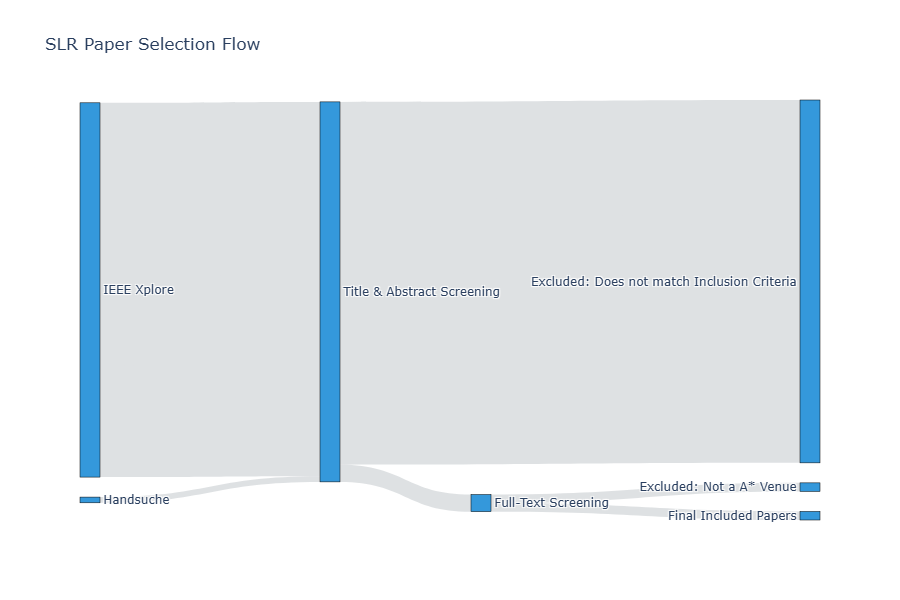
\includegraphics[width=1\linewidth]{images/selection_plot.png}
%     \caption{Auswahl der Arbeiten}
%     \label{fig:paper_selection}
% \end{figure}


\subsection{Überblick über das Korpus}

Aus den verbleibenden Arbeiten ergeben sich zunächst 5 verschiedene Benchmarks und 12 Arbeiten aus dem direkten Umfeld der Generierung von Quellcode. \todo{Ausbauen}

\section{Anforderungen als Eingabe}\label{ch:Anforderungen als Eingabe}

Diese Sektion befasst sich mit den spezifischen Eingabeartefakten, welche in den analysierten Arbeiten vorkommen. Das Format der Eingabe hat maßgeblichen Einfluss auf dessen Ausgabe. Schließlich lässt eine Formulierung in NL eine große Varianz and Detailgrad und technischem Inhalt zu, welcher wiederum Einfluß auf das Gesamtsystem hat. Ferner ergibt sich hier auch ein Einfluß auf die Autonomie des Systems.

\subsection{Kategorisierung der Eingabeformate}\label{ch:Kategorisierung der Eingabeformate}

Bevor die genauen Ergebnisse in Hinsicht auf die Eingaben vorliegen, lohnt es sich, eine formelle Kategorisierung von Eingabetypen vorzunehmen. Aus den analysierten Arbeiten lassen sich folgende distinkte Kategorien ableiten:

\begin{enumerate}
    \item \textbf{Unstruktuturierte Natürliche Sprache} \\ Einfache textuelle Beschreibungen, unformatierte Prompts
    \item \textbf{Strukturierte / Agile Artefakte} \\ Standartisierte Formate, z.B. User Stories
    \item \textbf{Formalisierte Anforderungen} \\ Ansätze bei denen initiale Anforderungen (aus einer anderen Kategorie) vor der tatsächlichen Eingabe (durch Verwendung von LLMs) formalisiert / diskutiert werden
    \item \textbf{Skizzen und erweiterte Repräsentatione}n \\ Eingaben die aus strukturierten Formatten bestehen, z.B. JSON
    \item \textbf{Test-basierte Eingaben} \\ Nutzung von Testfällen als Anforderungsspezifikation, ähnlich TDD\todo{oben erläutern oder hier oder weg lassen}
\end{enumerate}\todo{Hier noch Survey mit ins Spiel bringen falls dieser andere/bessere Befunde hat}

\subsection{Analyse der Eingabekategorien}\label{ch:Analyse der Eingabekategorien}

% \todo[inline]{Jede Kategorie als subsubsection, dann referenzieren mit den citations aus der Matrix und kurzer Erklärung was genau gemacht wurde, insofwern Abweichung der Definition oben besteht}

\subsubsection{Unstruktuturierte Natürliche Sprache}\label{ch:Analyse der Eingabekategorien:Unstruktuturierte Natürliche Sprache}



\todo[inline, color=blue]{ArchiLLM Analyse sucht noch einen Platz, hier passt es nicht gut hin.}
% \subsubsection{ArchiLLM}\label{ch:ArchiLLM}

% Die Forschungsfragen dieser Arbeit zielen vor allem auf die Präsentation von NL Anforderungen via User Stories ab. Wie bereits beschrieben, gibt es Stand heute praktisch keine Arbeiten, welche NL2Code via User Stories betrachten. Hier stellt \cite{calamoUserStoriesArchitectures2026} eine Ausnahme dar, weswegen diese Arbeit hier erwähnt wird.\todo{Formulierung Eröffnung anpassen}

% Die dabei vorgestellte Anwendung ''ArchiLLM'' schlägt einen neuen Ansatz vor, welcher bei der Entwicklung von Anwendungen die Zuverlässigkiet und Kohärenz erhöhnen soll. Zu diesem Zwecke stellt die Arbeit eine Pipeline vor:

% \begin{enumerate}
%     \item Extraktion von Microservices aus gegebenen User Stories
%     \item RAG Abfragen, gestützt durch Datensamlung zu Microservices Architecture
%     \item Generierung einer Architektur im JSON Format
%     \item Generierung einer Bare-Bones\todo{Begriff} Java Spring Boot Anwendung ohne implementierung von Anwendungs-Logik
% \end{enumerate}

% Trotz dieser [...] kann diese Arbeit leider im Rahmen dieser Arbeit nicht weiter betrachtet werden, da sie erhebliche Mengel mit sich bringt. Die Arbeit verifiziert ihre Ziele bzw. Aussagen nie gegen ihre Ergebnisse, es wird lediglich auf ein verlinktes Repository verwiesen. Die im Repository abgelegten Befunde und Auswertungen lassen sich allerdings nicht reproduzieren, da der gegebene Quellcode nicht ausführbar ist. Selbst nach Behebung von Fehler ergeben sich andere Zahlen als im Paper präsentiert. Die Methodik ist daher leider nicht nachvollziehbar und somit wird dieses Paper explizit nicht weiter verfolgt.

% In seinen Grundzügen ist die Arbeit allerdings trotzdem interessant für zukünftige Arbeiten: Sie präsentiert ein Datenmodell zur Evaluation von Ergebnissen, in denen User Stories von bestehenden studentischen Projekten gelabeled und jeweils bestimmten Microservices zugeordnet wurden. Dies eröffnet die Möglichkeit einer granularen Evaluation von generierten Microservices gegenüber der gegebenen Ground Truth.


\section{Ansätze zur Code-Generierung}\label{ch:Ansätze zur Code-Generierung}



\section{Evaluation in der Literatur}\label{ch:Benchmarks und Datensätze}

todo.

\subsection{Benchmarks}

\subsubsection{NL2Repo-Bench}

Bestehende Benchmarks evaluieren vor allem die Fähigkeiten von LLMs in der Generierung von lokalem Code oder auch die Reperatur von Code in geringeren Ausmaßen. Zur Evaluation von LLMs in einem größeren Kontext - der Exekution über größere Horizonte und näher an reellen Anwendungsbereichen aus der Softwareentiwcklung, präsentiert \cite{dingNL2RepoBenchLongHorizonRepository2026} den Benchmark $NL2Repo-Bench$. 

\todo[inline]{Vergleich nicht als paper/paper/paper sondern eher unter gemeinsamen Geischtspunknten. TODO: diese subsection entfernen und den Text in einen solchen Punk mit einarbeiten}


\section{Automatisierungsgrad}\label{ch:Automatisierungsgrad}



\section{Abgrenzung}\label{ch:Abgrenzung}\todo{Spezifizieren wie ich das am besten mache, siehe google doc letzte Konsultation (Notizen)}



\todo[inline,color=red]{AB HIER ALTER STAND ZUM RAUS KOPIEREN, DARÜBER NEUER STAND!}

% \todo[inline]{Einführung, Einordnung der Themengebiete im gröberem Kontext}

% \section{Anforderungsdokumente \& User-Stories}

% \todo[inline]{}

% \section{Datensätze zur Evaluation}

% \subsection{Evaluationsmetrkien}

% \subsection{Datensätze / Benchmarks}

% \section{Code Generierung}

% \todo[inline]{Zuerst Lösungs-übergreifende Erklärung, danach in die Details einzelner gewählter Lösungen}

% \subsubsection{Informationsbeschaffung wissenschaftlicher Literatur}

% Kernpunkt dieser Arbeit ist die Analyse von bestehenden Lösungen für \rqref{RQ1} und im erweiterten Rahmen auch \rqref{RQ2}. Neben den bereits angeführten Themenbereichen, sollen in dieser Sektion die tatsächlich existierenden Lösungsansätze für die Generierung von Quellcode aus Anforderungen analysiert werden. Um eine möglich umfangreiche Betrachtung durchführen zu können, muss demnach eine große Menge an wissenschaftlichen Arbeiten analysiert werden. In diesem Sinne bietet es sich an, eine ''Meta Analyse'', angelehnt an ein SLR (Structured Literature Review)\cite{kitchenhamGuidelinesPerformingSystematic2007} durchzuführen. 

% % Wie bereits angeführt soll im Ramen dieser Arbeit eine Analyse vorhandener Literatur stattfinden. Dabei ergeben sich Thematische Schwerpunkte welche der direkten Beanwortung der Forschungsfragen dienen:

% % \begin{itemize}
% %     \item Generierung von Quellcode aus Anforderungen
% %     \item Automatisierungsgrad von LLM (Multi-Agent) Systemen \textit{(für Quellcode Generierung)}
% % \end{itemize}

% % Weiterhin gibt es verschiedene Themenkomplexe welche durch ihre unmittelbare Nähe zu den Forschungsfragen \textit{oberflächlich} analysiert werden sollen:

% % \begin{itemize}
% %     \item Quellcode Generation durch Multi-Agent Systeme
% %     \item Generation von User Stories
% %     \item Generation von Tests (Unit, E2E, Integration, UAT)
% %     \item Evaluation von Ergebnissen (LLM-Judges, etc.)
% % \end{itemize}

% \subsubsection{Meta Analyse}

% % Hier soll zunächst die Outline für eine Meta Analyse definiert werden. Fokus der Analyse ist es, möglichst relevante wissenschaftliche Arbeiten zu sammeln und zu analysieren. Hinsichtlich des vorherigen Unter-Kapitels und in Betrachtung der Empfehlungen von \cite{kitchenhamGuidelinesPerformingSystematic2007} verfolge ich folgende Strategie:
% Das Ziel dieser Meta Analyse ist es, möglichst viele wissenschaftliche Arbeiten zum gegebenen Themenschwerpunkt zu sammeln und diese dann zu analysieren. Wie bereits erwähnt lehne ich mich hier an das Vorgehenes eines SLR\cite{kitchenhamGuidelinesPerformingSystematic2007} an und habe folgenden Durchführungsplan aufgestellt:

% \begin{enumerate}
%     \item Definition von Inklusions/Exklusions-Kriterien
%     \item Schlüsselwort Sammlung, daraus Queries definieren
%     \item Sammlung durch akademische Tools (IEEExplore, arXiv, etc.)
%     \item Bündelung und Sortierung von Ergebnissen
%     \item Filtern der Ergebnisse
% \end{enumerate}

% Nebene diesem groben, durch queries gestützen Prozess werden weiterhin auch händisch gefundene Arbeiten inkludiert. Für diese gelten allerdings die gleichen Kriterien.
% % Nach diesem Prozess sollten sich ca \textasciitilde 20 wissenschaftliche Arbeiten mit starker Relevanz ergeben.

% \subsubsection{Umsetzung Meta Analyse}

% \textbf{Strategie 1: SLR ähnliche Analyse via IEEExplore}

% \begin{enumerate}
%     \item Definition einer Query
%     \item Anwendung Inclusion Criteria (IC)
%     \item Anwendung Exclusion Criteria (EC)
%     \item Screening (Manual?=)
% \end{enumerate}

% \textbf{Query}

% Um möglichst viele Paper auf einmal zu gewinnen wird eine Query via IEEE Xplore ausgeführt. Hier wird bereits ein IC angewendet, da IEEE Xplore diese Funktionalität Diese sieht wie folgt aus:

% \begin{verbatim}
%     ("Large Language Model" OR LLM OR "Generative AI") 
%     AND ("User Story" OR Requirement) 
%     AND ("Code Generation" OR Autonomous OR "Multi-Agent")
% \end{verbatim}
% = 524 Arbeiten

% \textbf{Inclusion Criteria / Inklusionskriterien}

% \begin{enumerate}
%     \item Publikation zwischen 2023 und 2026
%     \item Arbeit behandelt die Transformation von natürlichsprachlich formulierten Anforderungen in Quellcode
%     \item Arbeit nutzt LLMs / Agentic Frameworks / Multi-Agent-Systeme
%     \item Arbeit evaluiert ihre Ergebnisse oder beschreibt die Architektur des Systems (am besten auch den Grad der Automatisierung)
% \end{enumerate}

% \begin{figure}
%     \centering
%     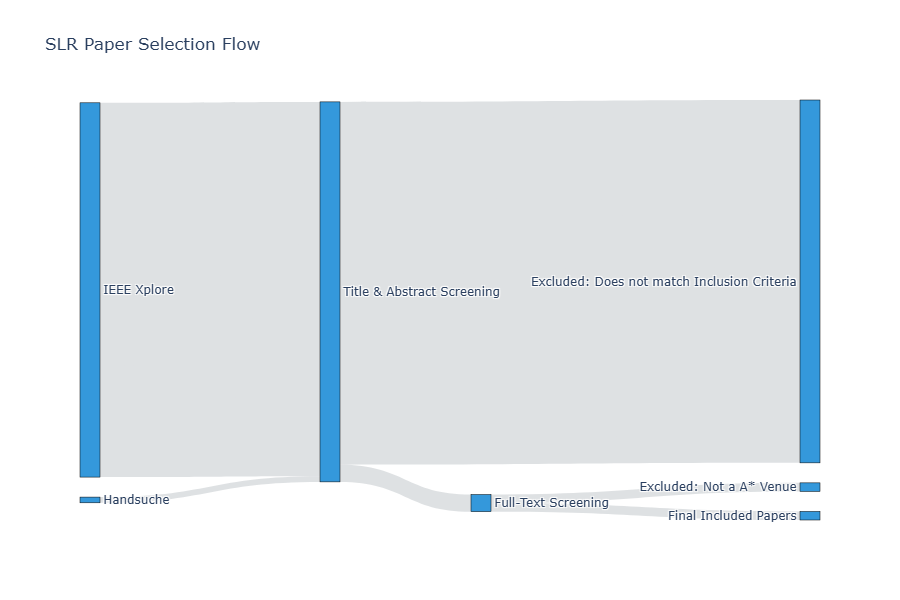
\includegraphics[width=1\linewidth]{images/selection_plot.png}
%     \caption{Auswahl der Arbeiten}
%     \label{fig:paper_selection}
% \end{figure}

% \section{Zusammenfassung}

% \begin{table}[t]
%     \todo[inline]{Summarize the properties, flaws, strengths, and weaknesses of all actually related publications here!}
%     \centering
%     \begin{tabular}{p{0.15\textwidth}|p{0.15\textwidth}|p{0.15\textwidth}|p{0.15\textwidth}|p{0.15\textwidth}}\hline\hline
%          & & & &  \\\hline\hline
%          & & & &  \\\hline
%          & & & &  \\\hline
%          & & & &  \\\hline
%          & & & &  \\\hline
%          & & & &  \\\hline
%          & & & &  \\\hline\hline
%     \end{tabular}
%     \caption{Overview of related work.}
%     \label{tab:placeholder}
% \end{table}

% #####################################################
% TODO: fragments that dont have a place yet
\todo[inline]{Text fragments I still need to sort under a section (more like subscetion)}
% #####################################################



\controlquestions{
Dieses Kapitel zeigt, welche wissenschaftlichen oder technischen Arbeiten es zu diesem Abschlussarbeitsthema bereits gibt, wie die Arbeit in diesen Kontext einzuordnen ist und welche Lücken geschlossen werden sollen.

\begin{itemize}
  \item {Einordnung des Themenumfelds}
  \begin{enumerate}
    \item Wurde beschrieben, welche Themenbereiche im Umfeld der eigenen Arbeit liegen (mit Begründung)? 
    \item Wurde das Umfeld der Arbeit qualifiziert und wissenschaftlich fundiert beleuchtet?
    \item Wird der aktuelle Forschungs- oder Entwicklungsstand zum Thema deutlich erkennbar gemacht?
  \end{enumerate}

  \item {Recherche und Auswahl der Literatur}
  \begin{enumerate}[resume]
    \item Wurden relevante Arbeiten systematisch und gezielt recherchiert (z.\,B.~über wissenschaftliche Datenbanken)?
    \item Deckt die Auswahl sowohl klassische (etablierte) als auch aktuelle Arbeiten ab?
    \item Sind die gewählten Arbeiten methodisch oder technisch mit der eigenen Arbeit vergleichbar?
    \item Wurden überwiegend wissenschaftliche Veröffentlichungen als Quellen angegeben?
    \item Wurden Quellen wie Wikipedia/Medium/Twitter/usw. explizit markiert und deren Vertrauenswürdigkeit diskutiert?
  \end{enumerate}

  \item {Inhaltliche Darstellung und Vergleich der Arbeiten}
  \begin{enumerate}[resume]
    \item Werden die Kernideen, Methoden und Ergebnisse der verwandten Arbeiten korrekt und prägnant dargestellt?
    \item Wurden die Stärken/Schwächen und idealerweise auch Chancen/Risiken (SWOT) der wichtigsten verwandten Arbeiten dargestellt?
    \item Wird deutlich, wie sich die verschiedenen Arbeiten inhaltlich oder methodisch voneinander unterscheiden?
    \item Welche Lücken existieren in den verwandten Arbeiten (liefert Rechtfertigung für die eigene Arbeit)? Wird transparent, was an bestehenden Arbeiten bereits gut funktioniert – und wo ihre Grenzen liegen?
    \item Werden die Arbeiten nicht einfach aufgezählt, sondern systematisch miteinander verglichen und diskutiert?
    \setcounter{lastenumcounter}{\value{enumi}}
  \end{enumerate}
\end{itemize}
}
\controlquestionscontinue{
\begin{itemize}
  \item {Ableitung und Abgrenzung der eigenen Arbeit}
  \begin{enumerate}[resume]\setcounter{enumi}{\value{lastenumcounter}}
    \item Wurde am Ende des Kapitels dargestellt, was der konkrete Fokus der eigenen Arbeit ist (mit Begründung)?
    \item Wurde klargestellt, was wiederverwendbar ist (als Konzept, Methode oder Tool)?
    \item Ergibt sich aus der Darstellung der verwandten Arbeiten ein logischer Übergang zur eigenen Problemstellung oder Motivation?
    \item Wurde im letzten Abschnitt eine Einordnung vorgenommen, welche Arbeiten die höchste Bedeutung für das eigene Thema haben?
    \item Wurde im letzten Abschnitt präzise hergeleitet, warum die eigene Arbeit gerechtfertigt ist, d.\,h. warum eine Forschungslücke existiert?
    \item Wird erläutert, wie die eigene Arbeit sich von den verwandten Arbeiten abgrenzt oder diese ergänzt?
    \item Wird klar, welchen wissenschaftlichen oder praktischen Mehrwert die eigene Arbeit im Vergleich bietet? Dies ist die Herleitung für die eigene konkrete Themenabgrenzung.
  \end{enumerate}

  \item {Zitierweise und Quellenqualität}
  \begin{enumerate}[resume]
    \item Sind alle Aussagen zu den verwandten Arbeiten korrekt belegt und mit fundierten Quellen versehen?
    \item Wird auf die begutachtete (peer-reviewed) Originalquellen und nicht nur auf Sekundärliteratur verwiesen?
  \end{enumerate}

\end{itemize}

}
